\documentclass[11pt,a4paper]{article}

\usepackage[utf8]{inputenc}
\usepackage[T1]{fontenc}
\usepackage{lmodern}
\usepackage[margin=2.4cm]{geometry}
\usepackage{graphicx}
\usepackage{booktabs}
\usepackage{tabularx}
\usepackage{array}
\usepackage{enumitem}
\usepackage[font=small]{caption}
\usepackage{url}
\usepackage[hidelinks]{hyperref}
\usepackage{tikz}
\usetikzlibrary{positioning,arrows.meta}

\renewcommand{\arraystretch}{1.15}
\newcolumntype{L}{>{\raggedright\arraybackslash}X}
\setlength{\parskip}{0.45em}
\setlength{\parindent}{0pt}
\setlist{itemsep=1pt,topsep=2pt}
\graphicspath{{figures/}}
\renewcommand{\topfraction}{0.9}
\renewcommand{\bottomfraction}{0.8}
\renewcommand{\textfraction}{0.1}
\renewcommand{\floatpagefraction}{0.8}

\begin{document}

\begin{center}
{\Large Can AI-written data checks be trusted next to expert checks?}\\[0.4em]
{\large Thesis plan}\\[0.8em]
Tomash Oosterbaan\\
MSc Artificial Intelligence, University of Groningen\\
Graduation project with Avanade and Rabobank\\
October 2026, draft
\end{center}

\section{Summary}

Organisations check incoming data with validation rules: simple tests such as ``a loan amount must be positive'' or ``total assets must equal liabilities plus equity''. Experts spend a lot of time writing these rules. AI language models, the technology behind tools such as ChatGPT, can now write such rules in seconds. Nobody knows how often these AI-written rules are right, or whether they add anything to the rules experts already wrote.

This thesis measures that. We use four public sets of rules written by expert committees and regulators, in three domains: company financial reports in the United States and in Europe, American mortgage applications, and a global register of companies. Each set comes with an official or verifiable way to tell whether a rule works, which we call an answer key. Open-source AI models write rules, and we test them in three ways: against the answer keys, against errors we place in the data on purpose, and against real errors that we label together with professionals.

The thesis delivers three things: evidence on when AI-written rules can be trusted and when not; a method to select the few AI rules worth keeping; and a working tool that lets a data team test AI-written rules before adopting them. No bank data is used. The plan builds on two pilot studies done in September and October 2026.

\section{The problem in plain words}

Data from a new source is rarely ready for use. Before a bank uses it in reports, models or decisions, a data team checks it. Long Tran described this work at Rabobank as technical validation, business rules, monitoring thresholds and manual investigation of exceptions \cite{tran}. Supervisors expect this: the Basel Committee's principles for risk data (BCBS 239) and the European Central Bank's 2024 guide on risk data aggregation ask banks for accurate data and effective controls \cite{bcbs239,ecbrdarr}.

Writing good rules takes time and domain knowledge. An analyst can now ask a language model for checks and receive twenty rules within a minute. Some are useful. Others look reasonable but are wrong: they flag hundreds of correct numbers, or miss the errors they were meant to find. Asked again the next day, the model may write a different rule. A wrong rule is not harmless. It lets errors through, or it floods the team with false alarms, and every alarm costs an employee's time. A rule that nobody can explain is also hard to defend to an auditor.

So the team faces a simple question: the AI suggested twenty rules; which of them, if any, should we adopt? This thesis tries to give that question a measurable answer.

\begin{table}[htbp]
\centering
\small
\begin{tabularx}{\textwidth}{@{}p{3.2cm}L@{}}
\toprule
Term & Meaning in this plan \\
\midrule
Validation rule & A check that every record must pass, for example ``assets = liabilities + equity''. \\
Expert rule set & Rules written and approved by a committee or regulator, not by us. \\
Answer key (gold standard) & Cases for which the correct outcome of a rule is known, so we can score a rule. \\
Error injection & Changing values in a copy of real data on purpose, while recording what we changed. \\
Alert, false alarm & An alert is a record a rule flags. A false alarm is an alert on correct data. \\
Review budget & How many alerts a team can check per report or file, for example one. \\
Language model (LLM) & An AI model trained on large amounts of text and code that can write text and code. \\
Open-weight model & A language model whose files can be downloaded and run on one's own computer. \\
Contamination & The model may have seen a rule during training, which would make a test too easy. \\
Baseline & A simple method without AI, used to check whether AI does better than something cheap. \\
\bottomrule
\end{tabularx}
\caption{Key terms.}
\label{tab:terms}
\end{table}

\section{What earlier research says}

AI that writes data-quality rules. Several recent studies let language models write data-quality rules. LeDQeR generates rules for a data-quality tool and removes poor ones with four filters, scored on tables with labelled errors \cite{ledqer}. AuDQ uses several cooperating AI agents and lets people rate the rules; its authors note that their datasets have no reference rule set to compare against \cite{audq}. Akella et al.\ generate rules and code with extra retrieved knowledge and present each rule on a readable card \cite{akella}. A master's thesis at TU Wien generated rules with GPT models and compared them with five to ten ``golden rules'' per dataset chosen by domain experts, checking by hand whether each golden rule was covered; 71 to 100\% were \cite{schneider}. Alexander et al.\ compared generated tests with one suite written by a single data scientist and ran each setup five times \cite{alexander}. Commercial data-quality tools are starting to offer this feature \cite{rehberger}.

How to choose among generated checks. Generating many candidate checks is easy; choosing the few worth keeping is the hard part. SPADE generates checks for AI pipelines and selects a small set that still catches the known failures while keeping false failures under a limit \cite{spade}. Auto-Validate learns checks from data and controls their false-alarm rate \cite{autovalidate}. Deequ suggests checks from simple data profiles \cite{deequ}. A warning comes from Martin et al., who showed that automatically discovered rules are mostly false \cite{martin}. None of these selection methods takes into account the rules a team already has.

AI on financial reports. Benchmarks such as FinTagging, FinAuditing and SEC-FinTables test whether language models can tag, audit or spot inconsistencies in company reports \cite{fintagging,finauditing,secfintables}. Models do reasonably well at finding numbers and poorly at the arithmetic relations between them. In these studies the model acts as a judge of the data, not as a writer of rules. Errors in such reports are common and have been studied since the early years of digital filing \cite{debreceny}.

Testing checks with planted errors. Software engineering tests test suites by planting small faults and counting how many the tests catch (mutation testing). The same idea has been used for data pipelines and data checks \cite{homayouni,jenga}, and Jung et al.\ describe realistic ways to plant errors in tables \cite{taberr}.

Two more points matter for the design. Rules for financial reports are written in a specialised language, and language models are known to perform worse on such less common languages \cite{joel}. Language models also give different code on different runs \cite{ouyang}, and they may have seen public rules during training; recent benchmarks therefore split test items by the date they were published \cite{livecodebench}.

The gap. We did not find a study that (1) scores AI-written rules against large, independent expert rule sets using their official answer keys, (2) measures what AI rules add beyond the expert rules a team already has, at a fixed review budget, or (3) checks the results on real errors labelled by people with domain knowledge. These three points define this thesis.

\section{What we did so far: two pilots and two short checks}

Table~\ref{tab:pilots} summarises the pilot work; the full report is available separately \cite{pilotreport}.

\begin{table}[htbp]
\centering
\small
\begin{tabularx}{\textwidth}{@{}p{2.3cm}LL@{}}
\toprule
Study & What we did & What we learned \\
\midrule
Pilot 1: which error detector? & Three public tables (credit card clients, bank marketing, wine). Planted five error types under three placement patterns in 990 scenarios. Compared simple rules and statistics with seven advanced detectors. & Simple rules caught every missing value, wrong type and invalid code. The best detector found 11 to 21 of 40 remaining errors but added 520 to 900 alerts per batch. Lesson: always compare with cheap methods and always count alerts. \\
Pilot 2: can AI-written rules be trusted? & US company reports (SEC) and the expert rules of the XBRL US Data Quality Committee (DQC). Two small open models wrote rules from the rule descriptions, from data samples and for gaps in the existing checks. & For rules published before the models, they found about 41\% of the official messages; for newer rules 3 and 13\%. Results varied strongly between runs. The best AI rule set caught 6 extra planted errors but gave 458 alerts per clean report, against 1.8 for the expert rules. \\
Mini-pilot & Three checks of the weak points of pilot 2. & No overlap between test and development companies. Giving the model the official code fixed 3 of 9 failed rules; most failures came from missing domain knowledge, not missing documentation. Selecting single AI rules against the existing checks left one rule with 3 extra catches at 0.2 alerts per report; a generic filter needed about twice the alerts. \\
EBA check & Could AI spot faulty rules in the European Banking Authority's rule set before they were switched off? & No useful signal: the AI scored worse than simply ranking rules by formula length. This direction was dropped. \\
\bottomrule
\end{tabularx}
\caption{Pilot work, September and October 2026.}
\label{tab:pilots}
\end{table}

\begin{figure}[htbp]
\centering
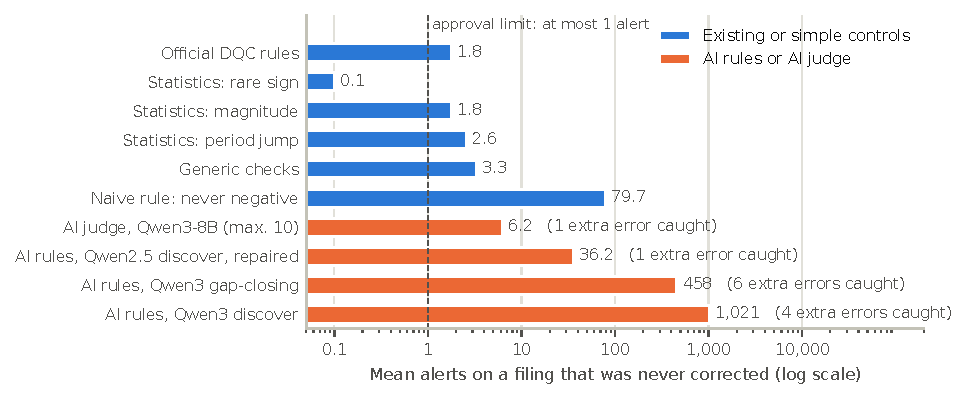
\includegraphics[width=0.92\textwidth]{fig_b_alerts.pdf}
\caption{Pilot 2. Mean alerts per report that was never corrected, on a log scale. In brackets: planted errors caught beyond the existing checks. AI rule sets caught a few extra errors at a very high alert cost.}
\label{fig:alerts}
\end{figure}

Three things change for the thesis. First, the pilots used two small models on a laptop processor; the thesis uses larger models on the university's computing cluster. Second, the pilots showed that missing domain knowledge is the main cause of failure, so the thesis tests whether giving the model that knowledge helps. Third, the pilots relied on planted errors and on one rule set; the thesis adds three more rule sets and a set of real errors labelled with professionals. All choices that were made after seeing results in the pilots, such as alert limits, will be fixed in advance.

\section{Research questions}

Main question: under what conditions can validation rules written by open-weight language models reproduce expert rules and add reliable detection value beyond expert controls, at a review cost a data team can accept?

\begin{description}[leftmargin=0pt,labelsep=0.5em]
\item[RQ1. Reproduce.] Given the written description of an expert rule, how often does a model write a rule that gives the same results as the official one, and how much does it help to give the model domain knowledge and the chance to test its own rule on example data?
\item[RQ2. Add and select.] What do AI-written rules catch that the existing expert rules and simple statistics miss, at what alert cost, and which selection method keeps the useful rules: no selection, a generic filter, a SPADE-like selection, or a selection that takes the existing expert rules into account?
\item[RQ3. Real errors and professional judgement.] Do the selected rules also catch real errors, labelled by people with domain knowledge, and do professionals agree with the rules the method selects?
\end{description}

Each question is answered on several datasets. If a result holds in US and European reports, in mortgage data and in company register data, it is more likely to hold for a bank's own data. If it holds in one domain only, that is also an answer.

Based on the pilots we expect that domain knowledge helps most for rules the models could not have seen, that the selection which takes existing rules into account gives more extra catches per alert than the others, and that real errors are harder to catch than planted ones. These are expectations to test, not claims.

\section{Datasets}

The thesis uses five datasets: four public datasets with expert rules, and a fifth that we build ourselves (Table~\ref{tab:data}). Each public dataset was chosen for four reasons: the data is public and free; the rules were written by experts independent of us; there is a way to score a rule; and the domain matters to a bank. A bank lends to companies and reads their financial reports, sells mortgages, and must identify the legal entities it deals with.

\begin{table}[htbp]
\centering
\footnotesize
\begin{tabularx}{\textwidth}{@{}p{2.6cm}p{3.2cm}LL@{}}
\toprule
Dataset & Rules and who wrote them & Answer key & Size (checked 31 October 2026) \\
\midrule
D1. US company reports (SEC, XBRL format) & DQC rules of the XBRL US Data Quality Committee, a committee of preparers, software firms and auditors \cite{dqc} & Official test cases: example reports with the exact messages each rule should give & 153 rules with test cases; 68{,}875 reports 2023 to mid-2025, of which 1{,}294 later corrected \cite{fsds} \\
D2. European company reports (ESEF) & ESEF data quality rules of XBRL International, the IFRS version of the DQC rules \cite{esefdqr} & Official IFRS test cases; official expected results for real European reports \cite{dqrconf} & 25 rules; 22 with 64 test reports; expected results for 1{,}739 reports (from 2022); 27{,}626 reports indexed \cite{esef} \\
D3. US mortgage applications (HMDA) & Edits of the US regulators FFIEC and CFPB in the Filing Instructions Guide \cite{hmda} & The regulator's own open-source implementation with its unit tests \cite{hmdaplatform} & About 300 edits (318 implementations: 237 validity, 72 quality, 9 syntax) with 330 test files; millions of public loan records per year \\
D4. Global company register (GLEIF, LEI) & 207 data quality checks of the Global Legal Entity Identifier Foundation, written as precondition and condition \cite{gleif} & No public answer per record; we build one (Section~\ref{sec:own}) & 207 checks in twelve quality criteria; public register of more than two million legal entities, updated daily \\
D5. Real errors (our own) & Not applicable & Corrections in US reports, labelled by the student and professionals & 300 corrected numbers, 100 labelled twice blind (target) \\
\bottomrule
\end{tabularx}
\caption{Datasets. Numbers for D1 to D4 were counted by us in the official repositories.}
\label{tab:data}
\end{table}

The four rule sets also differ in form: DQC and ESEF rules are written in a special rule language (XULE), the mortgage edits are plain-language descriptions with an official program behind them, and the GLEIF checks are semi-formal statements. This lets us see whether results depend on how rules are written.

Two cautions. The public mortgage data has been altered for privacy and has already passed the regulator's checks, so we test edits on planted errors and only use edits that can be evaluated on the public fields. The European expected results date from 2022, so we also regenerate them by running the official rules ourselves.

We considered and did not choose: the European Banking Authority's rules for bank reporting (the underlying bank reports are confidential, and our check found no signal for the question we could ask), and the classic research tables used for error detection (no expert rule sets).

\subsection{Gold standards we build ourselves}
\label{sec:own}

Real errors in company reports (D5). When a US company finds a mistake, it can file a corrected report. Comparing the two shows which numbers changed. In pilot 2 we checked 20 such changes: 9 were real errors in the original, 3 were not, and 8 were unclear; two separate AI passes agreed on only half. Corrections are therefore useful candidates but not yet a gold standard. We will build one. We draw 300 corrected numbers, spread over error kinds and companies, and write a short labelling guide with examples (tagging error, typing error, accounting restatement, not an error, unclear). The student labels all 300 using the original documents. Two professionals with accounting or XBRL knowledge, recruited through Avanade, Rabobank or the university's Faculty of Economics and Business, each label the same 100 without seeing other labels. We measure agreement with Cohen's kappa \cite{cohen} and discuss disagreements. The dataset contains public company information only and will be published if the participants agree. Involving professionals requires approval of the faculty ethics committee, which we will request in month one.

Answer key for the GLEIF checks (D4). GLEIF publishes the checks and monthly summary reports, but not the result per record. For 40 to 60 checks we write small test records directly from the specification, one that should pass, one that should fail and one where the check does not apply, and a reference implementation. A second person reviews both. As a sanity check we compare our failure rates with the figures in GLEIF's monthly reports.

Professional review of AI rules (RQ3). Three to five data-quality professionals review 30 to 40 AI rules each, with the evidence our tool produces, and decide whether they would adopt, reject or change each rule. We record their decision and the time it took, and compare it with the automatic selection.

\section{How we will answer the questions}

Preparation. Before the main experiments we write down the splits, alert budgets, metrics and approval criteria in a protocol and store it with a date. Data is split by company and by time, so that rules are never chosen and scored on the same reports. Rules are also split by publication date: rules published after a model's release are the fair test of whether it can write a rule it has not seen.

RQ1, reproduce. For every rule with an answer key, each model writes the rule in three conditions: (a) from the rule description only; (b) with domain knowledge added, for example whether an amount is a debit or credit, whether it is a balance or a flow, and how amounts add up; (c) as in (b), and the model may run its rule on development data and improve it, never on the answer key. Each rule is generated five times. All generated code runs in a closed sandbox. We measure the share of official messages a rule finds, the share of its own messages that are correct, whether the result is exactly right, and how much the five versions differ.

RQ2, add and select. We plant errors in reports and records that have no known errors: for example a flipped sign, a value multiplied by 1{,}000, one changed digit, a wrong item or category, swapped periods or a missing value. Where we have real corrections, the size of planted errors follows them. The existing controls are the official expert rules, built-in format checks and simple statistical checks learned from other data. Models then write rules for the errors these controls miss. We compare four selection methods, each choosing rules on one half of the data and being scored on the other half: no selection; a generic filter that keeps rules that run and are quiet on clean data, as in LeDQeR; a SPADE-like selection that balances catches and false alarms; and a selection that only keeps rules that catch errors the existing rules miss, within a fixed alert budget, and that are stable across generations. The main measure is the number of extra errors caught at a budget of 0.5, 1 and 2 alerts per report or file. As a second AI approach, a model also acts as a judge that reads a report and points at suspicious numbers.

RQ3, real errors and professionals. All controls and selected AI rules run on the real-error gold standard (D5) and on reports never corrected. We measure the share of real errors flagged and the alerts on clean reports, and we compare the professionals' decisions with the automatic selection.

Statistics. We report averages with 95\% confidence intervals from resampling over companies and rules, use paired comparisons where methods run on the same data, and report every run, including failed ones.

\section{Models}

We only use open-weight models (Table~\ref{tab:models}). This has four advantages. No data leaves the organisation, which matters for a bank. There are no usage costs. The exact model file can be stored, so results can be reproduced. And the release date is known, which we need for the contamination split. Large models run on the university's computing cluster, Hábrók; the tool itself must also work with a small model on an ordinary computer.

\begin{table}[htbp]
\centering
\small
\begin{tabularx}{\textwidth}{@{}p{4.4cm}p{1.9cm}L@{}}
\toprule
Model & Released & Why \\
\midrule
Qwen2.5-Coder 7B and 32B \cite{qwen25coder} & 2024 & Specialised in code; the 7B version was used in pilot 2, so results can be compared. \\
Qwen3 8B and 32B \cite{qwen3} & April 2025 & General model with reasoning; the 8B version was used in the pilots. \\
gpt-oss 20B and 120B \cite{gptoss} & August 2025 & A second model family, to check that conclusions do not depend on one company's models. \\
Newest open model at the start & To be fixed & Keeps the study current; fewer rules will be newer than this model, which we report. \\
\bottomrule
\end{tabularx}
\caption{Models. ``B'' is billions of parameters, a rough measure of model size.}
\label{tab:models}
\end{table}

Commercial models behind a paid service are not used, because of cost and because a bank would not send its data to them without approval. Every AI result is compared with methods that use no AI.

\section{Engineering artefact}

The pilots produced a working command-line tool, \texttt{dqstress}. In the thesis it becomes a workbench that follows the steps of a data team that adopts AI-written rules (Figure~\ref{fig:tool}).

\begin{figure}[htbp]
\centering
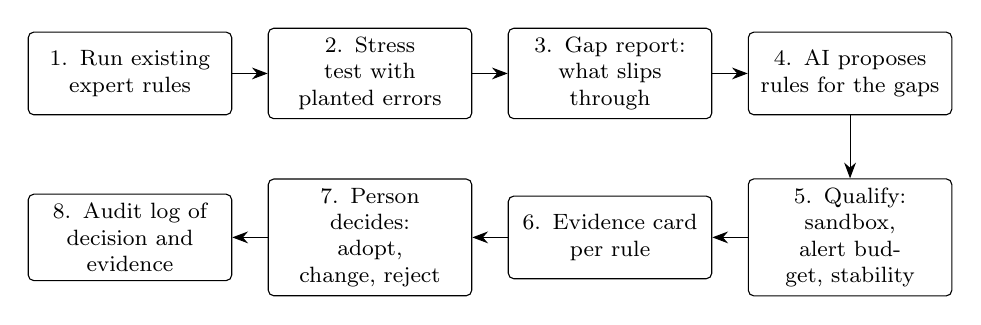
\begin{tikzpicture}[
  box/.style={draw, rounded corners=2pt, align=center, font=\footnotesize, minimum height=1.05cm, text width=2.35cm},
  arr/.style={-{Stealth[length=2mm]}}]
\node[box] (a) {1. Run existing\\ expert rules};
\node[box, right=0.45cm of a] (b) {2. Stress test with\\ planted errors};
\node[box, right=0.45cm of b] (c) {3. Gap report:\\ what slips through};
\node[box, right=0.45cm of c] (d) {4. AI proposes\\ rules for the gaps};
\node[box, below=0.8cm of d] (e) {5. Qualify: sandbox,\\ alert budget, stability};
\node[box, left=0.45cm of e] (f) {6. Evidence card\\ per rule};
\node[box, left=0.45cm of f] (g) {7. Person decides:\\ adopt, change, reject};
\node[box, left=0.45cm of g] (h) {8. Audit log of\\ decision and evidence};
\draw[arr] (a) -- (b); \draw[arr] (b) -- (c); \draw[arr] (c) -- (d);
\draw[arr] (d) -- (e); \draw[arr] (e) -- (f); \draw[arr] (f) -- (g); \draw[arr] (g) -- (h);
\end{tikzpicture}
\caption{The workbench. The tool never adopts a rule by itself and never changes data.}
\label{fig:tool}
\end{figure}

The evidence card shows, for each proposed rule, which planted errors it catches, which of those the existing rules already catch, how many alerts it gives on clean data, and whether repeated generations agree. For the team in the example, ``the AI suggested twenty rules'' becomes a short list of rules with evidence, of which perhaps none or a few are worth adopting.

The tool has an adapter for each data type in this study and one for ordinary tables, so a bank can run it internally on its own data and rules without sharing them. The language model sits behind a separate adapter, so an organisation can plug in the model it has approved. We evaluate the tool in three ways: every experiment in the thesis runs through it with one command, which makes the results reproducible; the professional review in RQ3 uses its evidence cards and measures decision time; and it is delivered with tests, documentation and an open-source licence.

\section{What could be new}

Much of this has been done before and we will not claim it: language models that write data-quality rules \cite{ledqer,audq,akella,schneider}, comparison with a small expert reference \cite{schneider,alexander}, selection of generated checks under a false-alarm limit \cite{spade,autovalidate}, human approval of rules \cite{audq}, planted errors to test checks \cite{homayouni,jenga}, and language models as judges of financial reports \cite{finauditing,secfintables}.

What we did not find, and what this thesis would add:
\begin{enumerate}
\item A test of AI-written rules against four large, independent expert rule sets, using their official or verified answer keys, with rules split by publication date to control for contamination. Earlier work used labelled tables, human ratings or five to ten reference rules.
\item A measurement of what AI rules add beyond the expert rules a team already has, at a fixed review budget, and a comparison of selection methods that do and do not take those existing rules into account.
\item A verified public set of real errors in company reports, labelled by people with accounting knowledge, and an answer key for the GLEIF checks. Both can be reused by others.
\end{enumerate}

Running the same protocol on four datasets is not a novelty in itself; the protocol stays the same on purpose, so that results can be compared, as one uses the same thermometer in different rooms. What is new is the evidence it produces: whether the answers hold across domains and jurisdictions. The novelty lies in the evaluation design, the selection method and the new gold standards, not in a new AI model. This is a fast-moving field (LeDQeR and AuDQ appeared in September and October 2026), so the literature will be checked again every month.

\section{Planning}

\begin{table}[htbp]
\centering
\small
\begin{tabularx}{\textwidth}{@{}p{1.4cm}L@{}}
\toprule
Month & Work \\
\midrule
1 & Literature update; protocol fixed and stored; ethics request; access to the computing cluster; labelling guide; contact professionals. \\
2 & RQ1 on D1 (US reports); GLEIF answer key built (D4). \\
3 & RQ1 on D2, D3 and D4; start labelling real errors (D5). \\
4 & RQ2 on D1: planted errors, AI rules for the gaps, four selection methods. \\
5 & RQ2 on D2 and D3; professional labelling of D5 finished. \\
6 & RQ3: real errors and professional review of AI rules; workbench completed. \\
7 & Analysis across datasets; demonstration to Avanade and Rabobank. \\
8 to 9 & Writing; buffer for delays. \\
\bottomrule
\end{tabularx}
\caption{Nine-month plan.}
\label{tab:plan}
\end{table}

D1 and D5 are the core. If time runs short, we cut in this order: GLEIF (D4) to RQ1 only, then the number of models, then the depth of RQ2 on D3.

\section{Risks}

\begin{table}[htbp]
\centering
\small
\begin{tabularx}{\textwidth}{@{}LL@{}}
\toprule
Risk & What we do about it \\
\midrule
AI rules add little even with larger models & The thesis is a measurement; a clear ``no, and this is why'' is a valid answer. \\
Few rules are newer than the models & Report confidence intervals; use rule sets with recent releases (DQC, HMDA). \\
Planted errors are not real errors & Base error sizes on real corrections; test on the real-error gold standard (D5). \\
Professionals have little time & Keep their part to about one day; the student labels everything, professionals label a shared subset. \\
Ethics approval takes long & Request it in month one; the public datasets do not depend on it. \\
Cluster access or queue delays & Start early; the small models from the pilots run on a laptop as fallback. \\
\bottomrule
\end{tabularx}
\caption{Main risks.}
\label{tab:risks}
\end{table}

\section{Value for Avanade and Rabobank}

The thesis gives a data team three things it can use without sharing any data: evidence on what to expect from AI-written rules, a procedure to decide which ones to adopt, and a tool that produces the evidence an auditor would ask for. Because the tool runs locally with an open model and its own adapters, it can be tried on internal data and internal rules after the thesis, under the bank's own approval process.

\begin{thebibliography}{99}
\small
\setlength{\itemsep}{1pt}
\setlength{\parskip}{0pt}

\bibitem{tran} L. Tran, correspondence with the author, 4 September 2026 (unpublished; observations specific to his working context).

\bibitem{bcbs239} Basel Committee on Banking Supervision, ``Principles for effective risk data aggregation and risk reporting,'' Bank for International Settlements, January 2013.

\bibitem{ecbrdarr} European Central Bank, ``Guide on effective risk data aggregation and risk reporting,'' May 2024.

\bibitem{ledqer} A.-C. Glock, T. H\"utter, J. F\"urnkranz, W. W\"o{\ss}, A. Dominka-Kiss, and L. Ehrlinger, ``Data Quality Rule Generation with LLMs,'' arXiv:2609.06053, 2026.

\bibitem{audq} J. Biggiogera, N. Colombo, K. Saxena, B. Sarmah, and S. Pasquali, ``AuDQ: Auditable Data Quality through Agentic Rule Discovery,'' arXiv:2610.26031, 2026.

\bibitem{akella} A. Akella, A. Kaul, K. Narayanam, and S. Mehta, ``Quality Assessment of Tabular Data using Large Language Models and Code Generation,'' Proceedings of EMNLP 2025: Industry Track, pp. 2713--2748, 2025. doi:10.18653/v1/2025.emnlp-industry.183.

\bibitem{schneider} A. Schneider, ``Template-Guided Rule Generation and Evaluation for Data Quality,'' MSc thesis, TU Wien, 2025. Supervisor G. Gottlob.

\bibitem{alexander} R. Alexander, L. Katz, C. Moore, M. W.-C. Wong, and Z. Schwartz, ``Evaluating the Decency and Consistency of Data Validation Tests Generated by LLMs,'' arXiv:2310.01402, 2023.

\bibitem{rehberger} T. Rehberger, T. H\"utter, L. Ehrlinger, and W. W\"o{\ss}, ``Evaluating Data Quality Tools: Measurement Capabilities and LLM Integration,'' arXiv:2604.09163, 2026.

\bibitem{spade} S. Shankar, H. Li, P. Asawa, M. Hulsebos, Y. Lin, J. D. Zamfirescu-Pereira, H. Chase, W. Fu-Hinthorn, A. G. Parameswaran, and E. Wu, ``SPADE: Synthesizing Data Quality Assertions for Large Language Model Pipelines,'' arXiv:2401.03038, 2024.

\bibitem{autovalidate} J. Song and Y. He, ``Auto-Validate: Unsupervised Data Validation Using Data-Domain Patterns Inferred from Data Lakes,'' Proceedings of SIGMOD, 2021.

\bibitem{deequ} S. Schelter, D. Lange, P. Schmidt, M. Celikel, F. Biessmann, and A. Grafberger, ``Automating Large-Scale Data Quality Verification,'' Proceedings of the VLDB Endowment, vol. 11, no. 12, pp. 1781--1794, 2018. doi:10.14778/3229863.3229867.

\bibitem{martin} A. Martin, E. C. de Almeida, O. Romero, and A. Queralt, ``How and Why False Denial Constraints are Discovered,'' Proceedings of the VLDB Endowment, vol. 18, no. 10, pp. 3477--3489, 2025. doi:10.14778/3748191.3748209.

\bibitem{fintagging} Y. Wang, L. Qian, X. Peng, et al., ``FinTagging: Benchmarking LLMs for Extracting and Structuring Financial Information,'' arXiv:2505.20650, 2025.

\bibitem{finauditing} Y. Wang, K. Wang, S. Yang, J. Patel, et al., ``FinAuditing: A Financial Taxonomy-Structured Multi-Document Benchmark for Evaluating LLMs,'' arXiv:2510.08886, 2025.

\bibitem{secfintables} S. Ke, Q. Wu, H. Li, and L. Cao, ``SEC-FinTables: Evaluating Large Language Models for Detecting Logical Inconsistencies on Tabular Data,'' Findings of ACL 2026, pp. 15587--15607, 2026. doi:10.18653/v1/2026.findings-acl.764.

\bibitem{debreceny} R. Debreceny, S. Farewell, M. Piechocki, C. Felden, and A. Gr\"aning, ``Does it add up? Early evidence on the data quality of XBRL filings to the SEC,'' Journal of Accounting and Public Policy, vol. 29, no. 3, pp. 296--306, 2010. doi:10.1016/j.jaccpubpol.2010.04.001.

\bibitem{homayouni} H. Homayouni, S. Ghosh, and I. Ray, ``An Approach for Testing the Extract-Transform-Load Process in Data Warehouse Systems,'' Proceedings of IDEAS, pp. 236--245, 2018. doi:10.1145/3216122.3216149.

\bibitem{jenga} S. Schelter, T. Rukat, and F. Biessmann, ``JENGA: A Framework to Study the Impact of Data Errors on the Predictions of Machine Learning Models,'' Proceedings of EDBT, pp. 529--534, 2021.

\bibitem{taberr} P. Jung, S. J\"ager, N. Chandler, and F. Biessmann, ``Towards Realistic Error Models for Tabular Data,'' ACM Journal of Data and Information Quality, vol. 17, no. 4, article 28, 2025. doi:10.1145/3774914.

\bibitem{joel} S. Joel, J. J. Wu, and F. H. Fard, ``A Survey on LLM-based Code Generation for Low-Resource and Domain-Specific Programming Languages,'' ACM Transactions on Software Engineering and Methodology (accepted), arXiv:2410.03981.

\bibitem{ouyang} S. Ouyang, J. M. Zhang, M. Harman, and M. Wang, ``An Empirical Study of the Non-Determinism of ChatGPT in Code Generation,'' ACM Transactions on Software Engineering and Methodology, vol. 34, no. 2, 2025. doi:10.1145/3697010.

\bibitem{livecodebench} N. Jain, K. Han, A. Gu, W.-D. Li, F. Yan, T. Zhang, S. Wang, A. Solar-Lezama, K. Sen, and I. Stoica, ``LiveCodeBench: Holistic and Contamination Free Evaluation of Large Language Models for Code,'' Proceedings of ICLR, 2025. arXiv:2403.07974.

\bibitem{pilotreport} T. Oosterbaan, ``Data-quality controls with and without AI: what two pilot studies showed,'' project repository \texttt{masterthesis\_direction3\_pilot}, October 2026.

\bibitem{dqc} XBRL US Data Quality Committee, ``DQC rules (dqc\_us\_rules),'' rules, documentation and test suite, version 31. \url{https://github.com/DataQualityCommittee/dqc_us_rules}

\bibitem{fsds} U.S. Securities and Exchange Commission, ``Financial Statement Data Sets,'' quarters 2023q1 to 2025q2. \url{https://www.sec.gov/data-research/sec-markets-data/financial-statement-data-sets}

\bibitem{esefdqr} XBRL International, ``ESEF Data Quality Rules.'' \url{https://esef-dqr.xbrl.org}

\bibitem{dqrconf} XBRL International, ``ESEF DQR Conformance Suite.'' \url{https://gitlab.xbrl.org/xii/dqr-conformance}

\bibitem{esef} XBRL International, ``filings.xbrl.org,'' public repository of ESEF filings. \url{https://filings.xbrl.org}

\bibitem{hmda} Federal Financial Institutions Examination Council and Consumer Financial Protection Bureau, ``Filing Instructions Guide for HMDA data collected in 2025.'' \url{https://ffiec.cfpb.gov/documentation/fig/2025/overview}

\bibitem{hmdaplatform} Consumer Financial Protection Bureau, ``HMDA Platform,'' open-source filing and validation software. \url{https://github.com/cfpb/hmda-platform}

\bibitem{gleif} Global Legal Entity Identifier Foundation, ``Data Quality Rule Setting,'' version 3.5, and monthly data quality reports. \url{https://www.gleif.org/en/lei-data/gleif-data-quality-management}

\bibitem{cohen} J. Cohen, ``A Coefficient of Agreement for Nominal Scales,'' Educational and Psychological Measurement, vol. 20, no. 1, pp. 37--46, 1960.

\bibitem{qwen25coder} B. Hui, J. Yang, Z. Cui, J. Yang, et al., ``Qwen2.5-Coder Technical Report,'' arXiv:2409.12186, 2024.

\bibitem{qwen3} A. Yang, A. Li, B. Yang, B. Zhang, et al., ``Qwen3 Technical Report,'' arXiv:2505.09388, 2025.

\bibitem{gptoss} OpenAI, ``gpt-oss-120b \& gpt-oss-20b Model Card,'' arXiv:2508.10925, 2025.

\end{thebibliography}

\end{document}
